\section{Présentation du fonctionnement de la Plateforme de Service}

\subsection{Architecture de la plateforme }

La plateforme Cordys fonctionne en trois mandants.
\vspace{4mm}
\begin{itemize}
	\item Mandant de Production
	\item Mandant de Test (ou Acceptance)
	\item Mandant de Développement
\end{itemize}
\vspace{4mm}

Les utilisateurs ``classiques" n'ont accès qu'au mandant de production, c'est ce dernier le plus important: il contient les données Business de l'entreprise.

Les développeurs d'applications sur la plateforme Cordys peuvent accéder à l'environnement de test qui est une réplication complète de l'environnement de production (en terme de services et logiciels en place). Il est essentiel de tester une application dans ce mandant avant de la déployer en production de sorte à vérifier la compatibilité avec le futur environnement. Cette étape est absolument nécessaire du fait de l'impossibilité d'altération ou suppression des données Business et stratégiques dans ce mandant.

Concernant le mandant de développement, c'est le seul mandant qui n'est pas rattaché aux services Valeo, Google et LDAP. Ce dernier est uniquement là pour développer et tester les applications de manière succincte  avant de les soumettre à validation.


Nous suivons donc un Workflow de développement de type DTAP : Development, Testing, Acceptance and Production : 

\begin{enumerate}
	\item Une fois que le développeur pense que l'application est prête, elle est copiée dans l'environnement de test pour vérifier qu'elle fonctionne comme attendue.\\
	Les tests ne sont pas normalisés comme ils devraient l'être dans un Workflow de type DTAP. Il appartient à chaque développeur de s'assurer du fonctionnement de son application.\\
	 \item Une fois les tests positifs, l'application est passée en revue avec le ``Business Owner" de la future application (celui qui sera responsable de cette application et des données Business qui y transiterons). Ce dernier vérifiera que l'application correspond bien à son besoin. \\
	 \item Après l'acceptation de l'application par le ``Business Owner", l'application est déployée en production et rendue accéssible.
\end{enumerate}

 \begin{figure}[H]
    \centering
    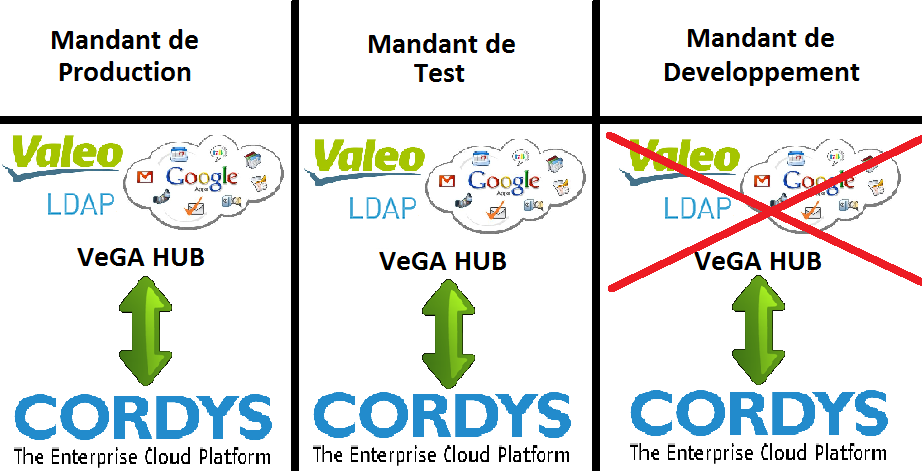
\includegraphics[height=9.25cm]{architecture_Cordys.png}
	\caption{\textit{Schéma de l'architecture Cordys chez Valeo}}\label{image.architectureCordys} 
\end{figure}

\clearpage

\subsection{Présentation de l'interface standard d'une application}


L'interface d'une application Cordys est relativement identique quelque soit l'application.\\
Ainsi, quel que soit l'application, deux onglets sont systématiquement disponibles : \textit{My Page \& Setup}.
Le nom de l'application se situe en haut à gauche, se qui constitue un bon repère visuel.\\
En plus de celà, un menu déroulant ``Change Application", permet d'afficher la liste entière des applications auxquelles vous avez le droit d'accéder.

 \begin{figure}[H]
    \centering
    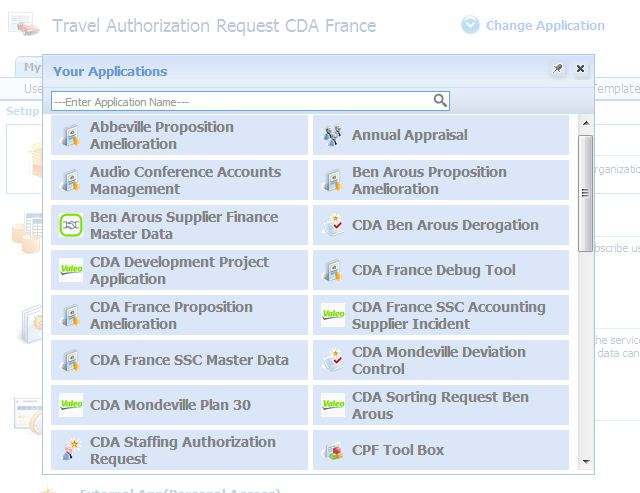
\includegraphics[height=6cm]{cordysChangeApplication.jpg}
	\caption{\textit{Interface Standard d'une application Cordys - Menu ``Change Application"}}\label{image.CordysChangeApplication} 
\end{figure}

\subsubsection{L'onglet My Page}

La vue par défaut d'une application est l'onglet: ``My Page". Il regroupe les dernières données relatives à l'utilisateur.

 \begin{figure}[H]
    \centering
    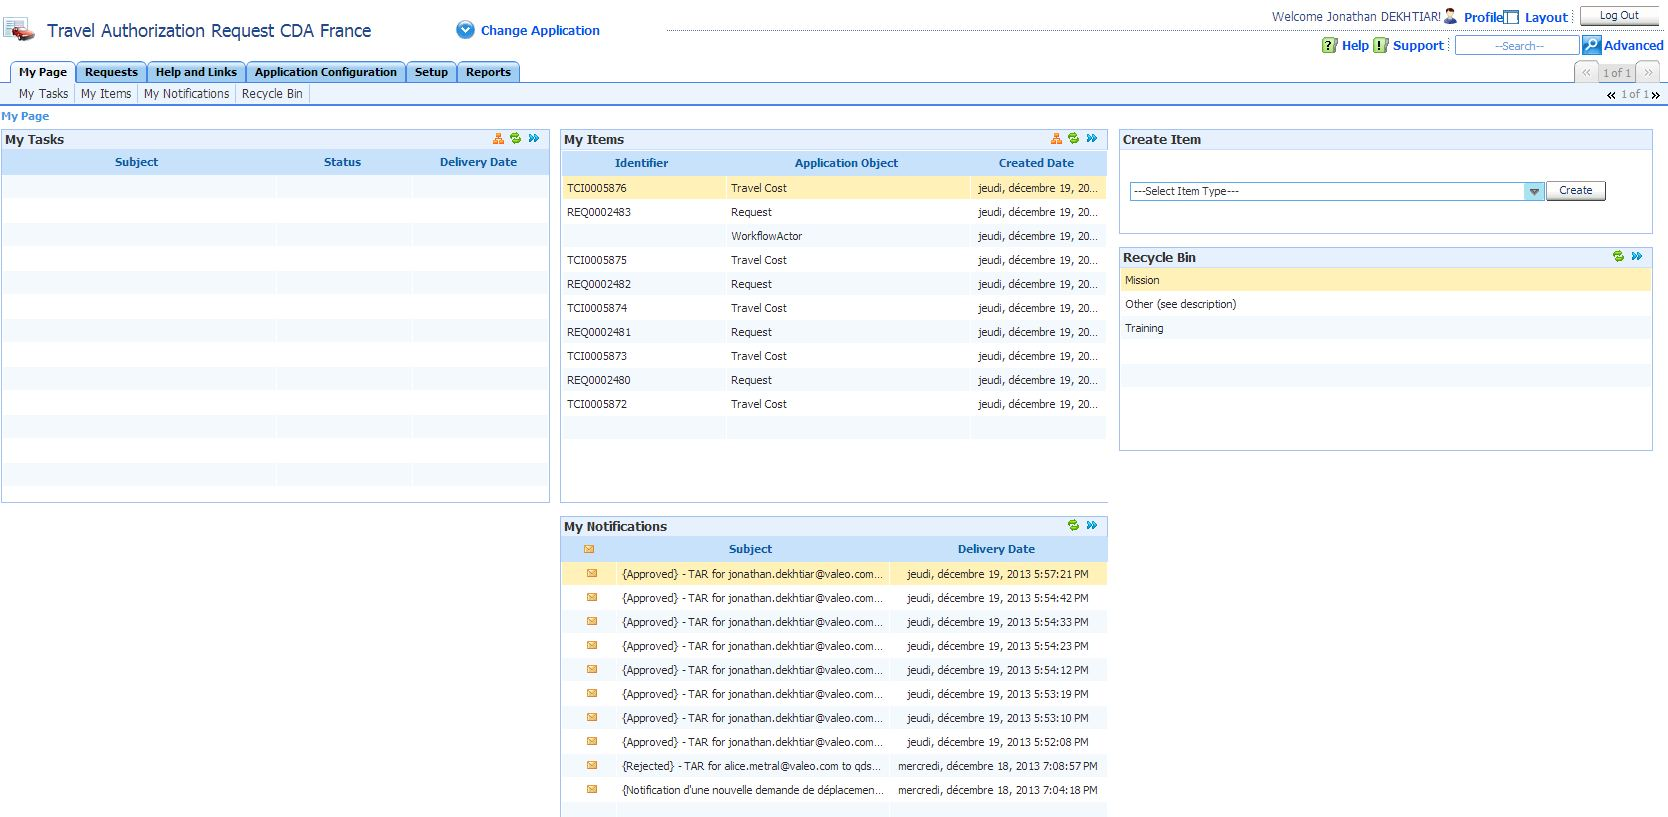
\includegraphics[height=8cm]{cordysMyPage.jpg}
	\caption{\textit{Interface Standard d'une application Cordys - Onglet ``My Page"}}\label{image.CordysMyPage} 
\end{figure}

\subsubsection{L'onglet Setup}

L'onglet Setup varie en fonction des droits d'accès. Un utilisateur aura accès uniquement à la personnalisation de son interface (de manière assez restreinte) et l'administrateur pourra, lui, accéder à plusieurs rubriques permettant l'import de données dans l'application, l'analyse des processus en cours d'éxécution, les tâches actuellement en attentes (et les réaffecter si nécessaire), la liste des utilisateurs de l'application et leurs droits respectifs (en lecture et en modification), ainsi que d'autres fonctions moins utiles comme les modèles d'emails ou l'état des nombres auto-incrémentés.

 \begin{figure}[H]
    \centering
    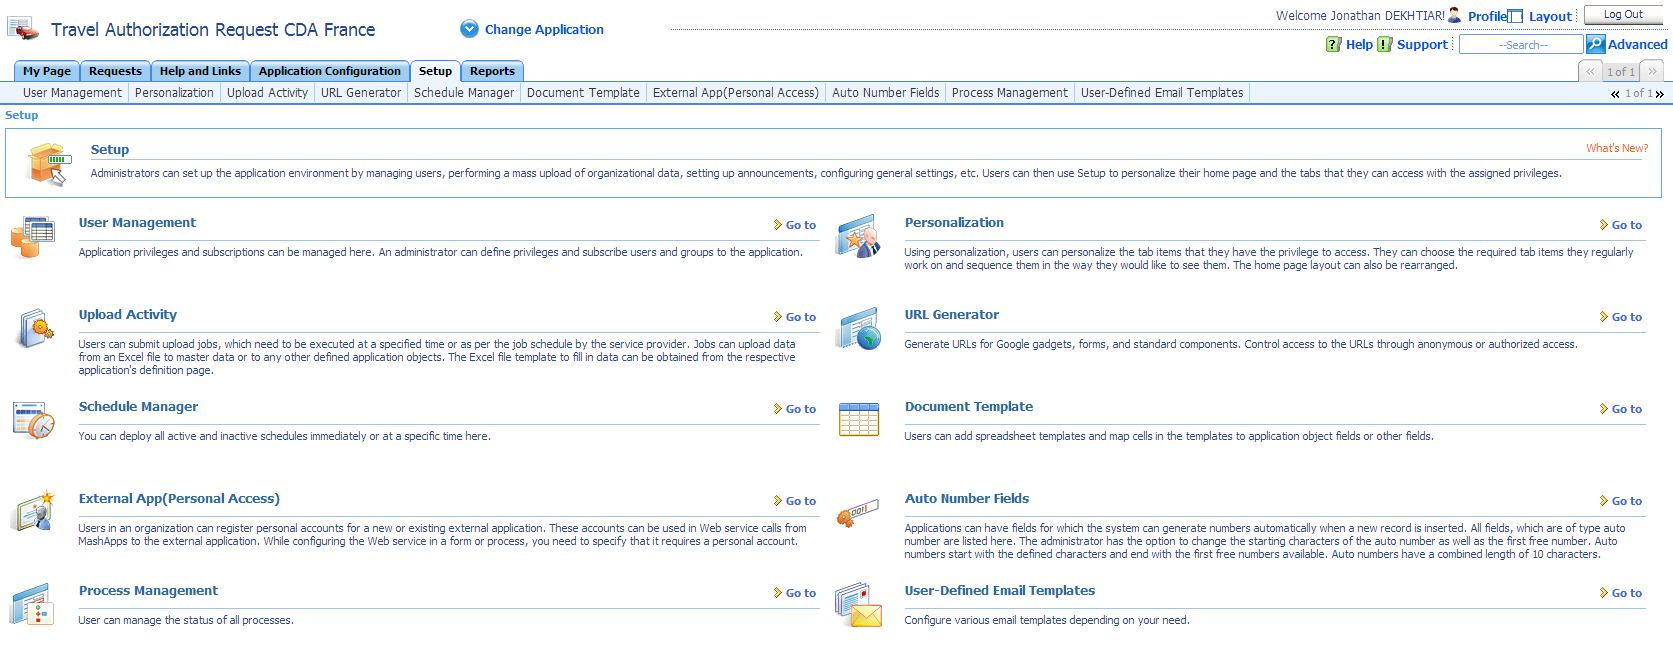
\includegraphics[height=7cm]{cordysSetupAdmin.jpg}
	\caption{\textit{Interface Standard d'une application Cordys - Onglet ``Setup" - Vue Administrateur}}\label{image.CordysSetupAdmin} 
\end{figure}

 \begin{figure}[H]
    \centering
    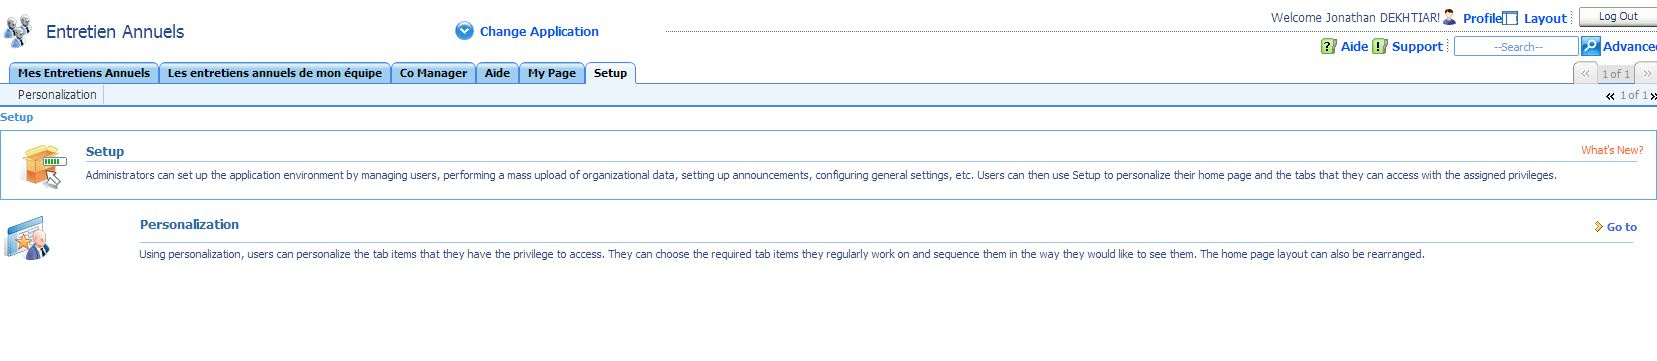
\includegraphics[height=3.8cm]{cordysSetupUser.jpg}
	\caption{\textit{Interface Standard d'une application Cordys - Onglet ``Setup" - Vue Utilisateur}}\label{image.CordysSetupUser} 
\end{figure}

\clearpage

\subsubsection{L'onglet Report}

L'onglet Report est automatiquement disponible pour chaque application, cependant l'administrateur peut choisir ou non de le faire apparaitre dans l'application et/ou de le rendre disponible uniquement pour une partie des utilisateurs ou pour tout le monde en modifiant les droits d'accès.

Les Reports sont à ``paramétrer" en développement pour qu'ils apparaissent en production de manière systématique. Sinon ``\emph{l'instant Report}" permet d'extraire des données de manière rapide et flexible. Il est cependant plus long à effectuer qu'un Report automatique et nécessite la connaissance du nom des champs que l'on veut extraire.

 \begin{figure}[H]
    \centering
    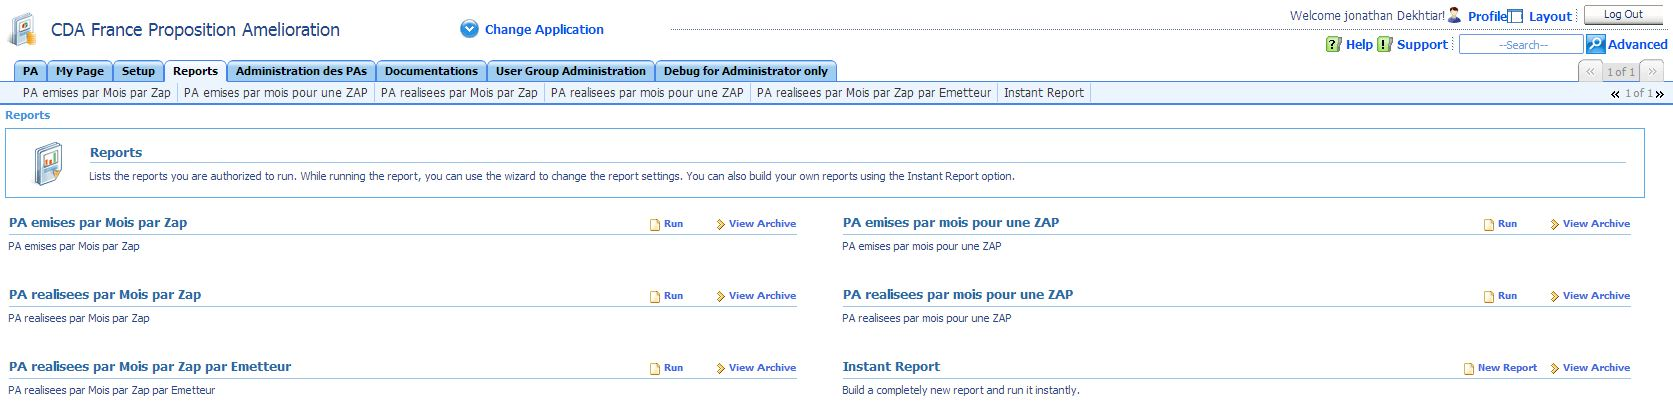
\includegraphics[height=3.8cm]{cordysReports.jpg}
	\caption{\textit{Interface Standard d'une application Cordys - Onglet ``Report"}}\label{image.CordysReports} 
\end{figure}

\clearpage

\subsection{Présentation de l'interface developpeur de Cordys}

\subsubsection{La page d'accueil de la plateforme de développement}

La page d'accueil de la plateforme de développement est assez sobre, on y retrouve les différentes sections sur la gauche et une vue ``graphique" au centre expliquant à quoi sert cet onglet. Toujours dans l'optique de permettre à un utilisateur, sans bagage informatique, de pouvoir mettre en place simplement et rapidement en place une application.

 \begin{figure}[H]
    \centering
    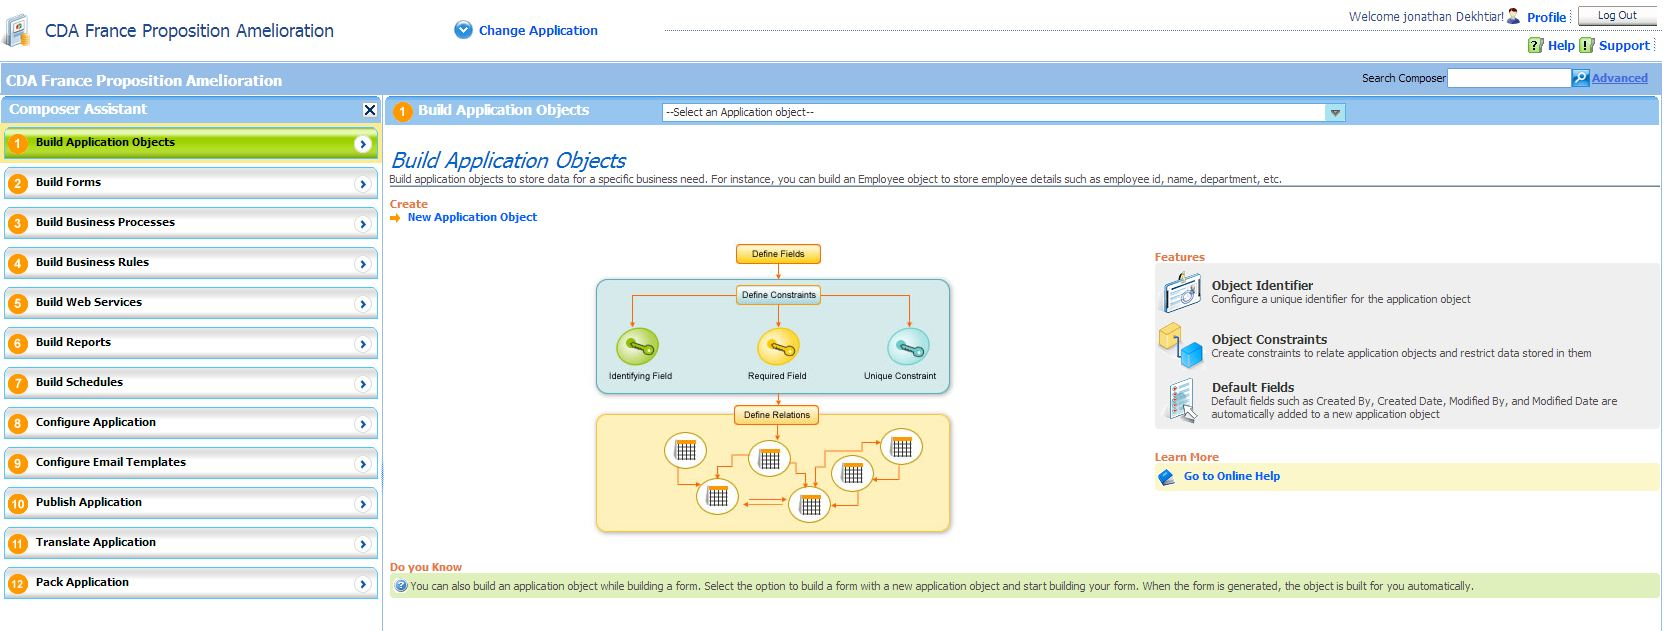
\includegraphics[height=6.9cm]{cordysDevHome.jpg}
	\caption{\textit{Interface de développement de Cordys - Page D'accueil}}\label{image.CordysDevHome} 
\end{figure}

\subsubsection{L'onglet ``Application Object"}

Un \emph{Application Object} est l'équivalent de ce qu'on appelle en programmation orientée objet : \textbf{un objet}.\\
Ces objets sont la base de l'application, ils sont à définir selon les besoins et donc selon le cahier des charges qui a été établi au préalable.\\
Des diagrammes UML sont donc à prévoir sur les applications lors de la définition du projet.

Les \emph{Application Objects} permettent de stocker les données relatives à l'entreprise. Par exemple, les dépenses de l'entreprise dans une application dédiée à la validation des factures ou au remboursement des frais des employés.

Afin de stocker des données dans un \emph{Application Object}, il est nécessaire d'ajouter donc des champs relatifs à l'utilisation (Exemple: FactureID, UserName, ApproverName, ...).

Lors de la création de l'\emph{Application Object}, il est possible de définir la clé primaire, des index afin de faciliter et accélerer la recherche et des contraintes (sur un ou plusieurs champs).

Tous les \emph{Application Object} sont stockés dans l' \emph{``Application Object Repository"}. Il est ainsi possible de les modifier, et de les supprimer par l'intermédiaire de ce répertoire.

 \begin{figure}[H]
    \centering
    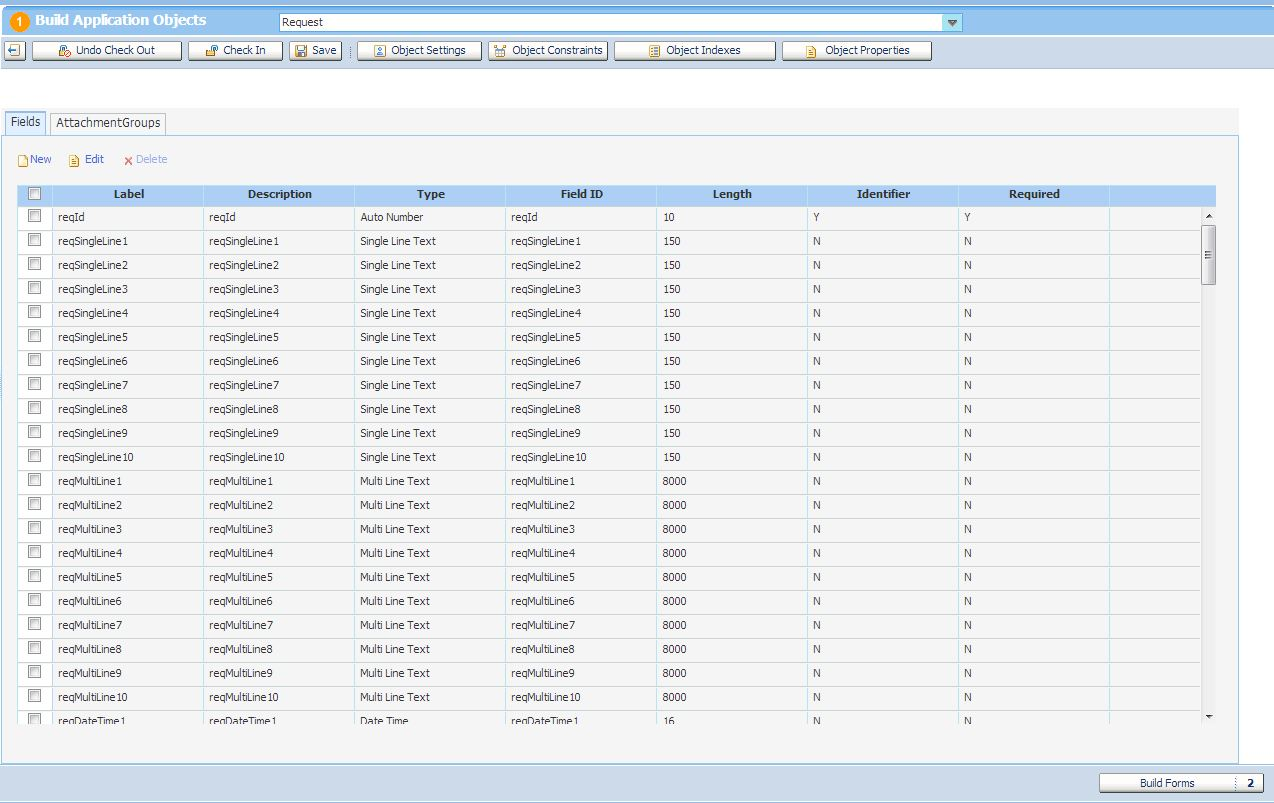
\includegraphics[height=11cm]{cordysDevAOForm.jpg}
	\caption{\textit{Interface de développement de Cordys - Interface de définition des Application Object}}\label{image.CordysDevAOForm} 
\end{figure}

\clearpage

\subsubsection{L'onglet ``Forms"}

Une fois un \emph{Application Object} défini, il est possible de créer un ou plusieurs formulaires de manière à permettre l'instanciation de ces objets. Tous les champs relatifs à cet \emph{Application Object} sont automatiquement ajoutés au formulaire, charge au développeur de choisir s'il désire tous les garder et de les agencer à sa convenance.\\
Il est également possible de créer un formulaire sans le rattacher à un \emph{Application Object}. Dans ce cas, il est impossible de sauvegarder les informations entrées dans ce formulaire et celles affichées par les différents Web-Services appelés.

Différents outils sont à disposition afin de mettre en place le formulaire répondant exactement aux attentes: 

\begin{itemize}\itemsep5pt
	\item \textbf{Les Types de Sections: }Il possible de créer différent types de section pour organiser les champs du formulaire. Ces sections portent le nom de : ``Group Box", ``Grid", et  ``Tab sections". Il est également possible de créer une section pour attacher un ou plusieurs fichiers et des éventuels commentaires.
		
	\item \textbf{Les types de Champs: }De nombreux types de champs sont à disposition des développeurs, le choix dépend alors du type d'information qui y sera stocké.
	
	\item \textbf{Le ``Repertoire" de Web Services: }Tous les Web services de l'application sont stockés dans un répertoire. Il est ainsi possible d'ajouter des Web Services, basés sur des Application Objects et Business Process, à un formulaire directement depuis ce répertoire. Il est également possible d'ajouter des Web Services ``externes" SOAP ou REST.
	
	\item \textbf{Les Paramètres de Formulaire: }Une des sources de flexibilité dans la création des formulaires vient de ce qu'on appel les ``Form Parameters" ou en Français : Les Paramètres de Formulaire. Ils permettent de définir quels champs seront les entrées ou les sorties d'un ou plusieurs Web Services.
	
	\item \textbf{Design adaptatif: }Les formulaires peuvent être créés de manière ``flexible" et s'adapter à la taille de la fenêtre ou du design établi (\textit{Responsive Design}). Les Sections, champs et Web Services peuvent être placés de manière quelconque dans le formulaire.
			
	\item \textbf{Les champs de type ``Lookup": }Il est possible de paramétrer des champs pour les associer à un ``\emph{lookup}". Cela leur permettra de \textbf{sélectionner} des données relatives à des Application Objects ou aux Utilisateurs (Groupes, Fonction, Email  ...).

	\item \textbf{Les règles de Formulaire: }Il est possible de définir des conditions qui vont modifier le comportement d'un formulaire en utilisant ce qu'on appelle une ``Règle de Formulaire". Il est ainsi possible d'assigner des valeurs, afficher des messages, cacher ou forcer l'affichage, bloquer ou débloquer un champs, une section.
	
	\item \textbf{Les vues: }Il est possible de créer des vues de manière à trier les données pour les formulaire de type tableau ou ``Grid" en anglais.
	
	\item \textbf{L'éditeur de Script: }Ce dernier module permet aux développeurs plus chevronnés d'avoir un contrôle total de leur formulaire avec l'aide du Javascript et un petite sur-couche \textit{made in Cordys}.

\end{itemize}

En dehors des fonctions citées plus haut, un système de versionnement est en place et permet d'afficher les dix dernières révisions de l'objet ou du formulaire via un système de ``Check In" / ``Check Out"  dans le but d'améliorer l'efficience et de réduire la maintenance. Il est également possible de modifier le formulaire de sauvegarder et de ne finalement rendre les modifications effectives que plusieurs jours après en effectuant le ``Check In" au bon moment.

Il est possible de prévisualiser le formulaire pendant son édition. Cette fonction permet de vérifier le bon comportement pendant l'exécution (en particulier les scripts et règles de formulaires).
\vspace{8mm}

\begin{figure}[H]
    \centering
    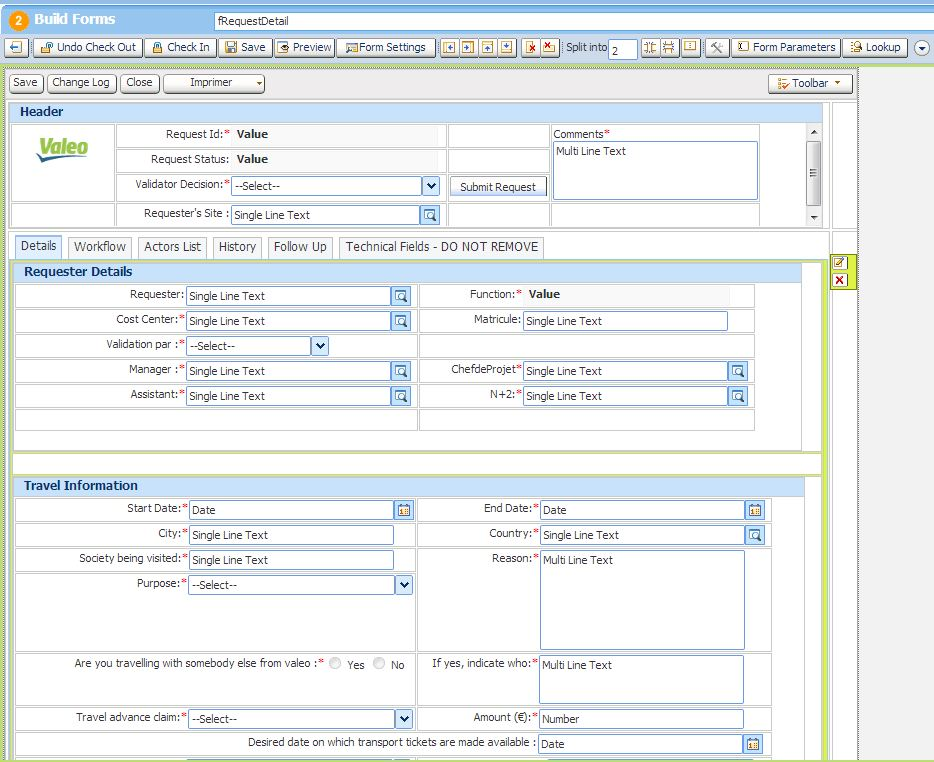
\includegraphics[height=14.5cm]{cordysDevFormsDef.jpg}
	\caption{\textit{Interface de développement de Cordys - Interface de définition des Formulaires}}\label{image.cordysDevFormsDef} 
\end{figure}

\clearpage
\subsubsection{L'onglet ``Business Process"}

C'est la notion clé du système Cordys, et d'ailleurs mon sujet de stage mentionne cet élément sous le nom de \textbf{Workflow}. Ce n'est donc pas un outil à proprement parlé mais plutôt une finalité: sa mise en place.

Un Business Process est donc un ensemble d'activités liées qui produisent un service de manière à atteindre les objectif du business. Les ``Business Processes" sont \textbf{la manière} d'effectuer une tâche spécifique au sein d'une organisation spécifique. 
Un Business Process définit, dans notre cas, un parcours de validation ou signature et ainsi aide les employés à interagir avec les différentes entités de l'entreprise.



Pour exemple, prenons l'approbation du remboursement d'une note de frais :

Un employé peut avoir des dépenses durant un voyage d'affaire et doit être remboursé. Ainsi il serait intéressant d'établir un \textbf{Business Process} décrivant le parcours de signature à effectuer de manière à donner l'autorisation de manière automatique à la finance pour le paiement de la note de frais:\\
Demande de remboursement => Validation du supérieur hiérarchique => Validation du chef de projet => Demande de remboursement validée. \\
Il peut être judicieux de notifier tout le monde dès l'acceptation ou le refus de la demande. Le remboursement peut ainsi être débloqué par le service financier.

Automatiser ce genre de processus permet d'une part de limiter les erreurs humaines et d'autres part d'en maximiser l'efficience et la traçabilité.

Un Business Process se définit par:

\begin{itemize}\itemsep7pt

	\item \textbf{Un But: } Un Business Process possède un but bien défini, qui est le besoin Business d'une action systématique.
	
	\item \textbf{Des données en ``entrée": }Un Business Process a besoin de données en entrée, que l'on appelle ``ressources", pour fonctionnner. Pour exemple, reprenons notre exemple de la validation des notes de frais. Voici quelques ressources : Date du début du Voyage, Date de fin du voyage, montant de la note de frais, Utilisateur demandeur ...
	
	\item \textbf{Des données en ``sortie: "}Un Business Process produit une ou plusieurs sorties qui fournissent des informations importantes pour l'entreprise.
	
\end{itemize}

Il est possible de publier un Business Process et de l'intégrer à un formulaire à la manière d'un Web Service. Il est ensuite possible de définir les ``déclencheurs" qui vont appelés le Business Process à intervalle régulier ou sous certaines conditions.

\begin{figure}[H]
    \centering
    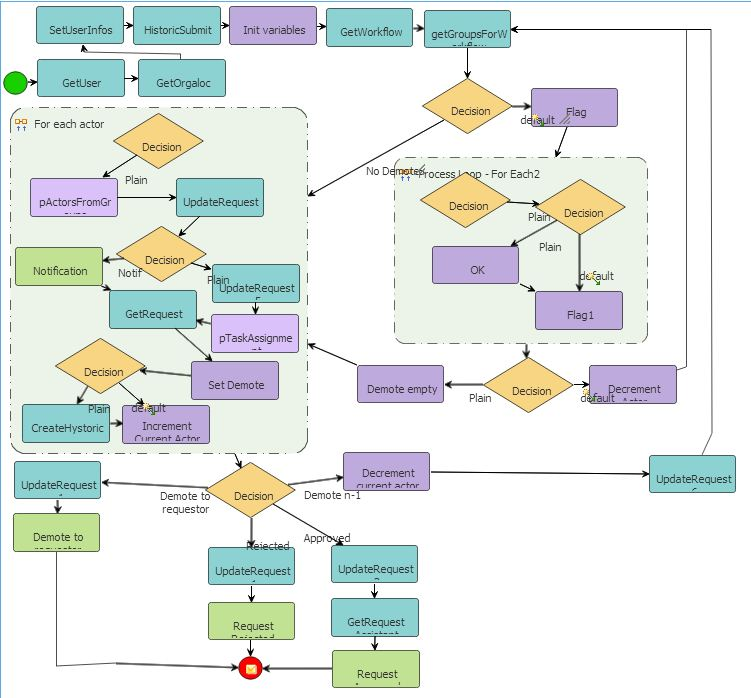
\includegraphics[height=17cm]{cordysDevBusinessProcess.jpg}
	\caption{\textit{Interface de développement de Cordys - Exemple d'un Business Process}}\label{image.cordysDevFormsDef} 
\end{figure}

\clearpage

\subsubsection{L'onglet ``Business Rules"}

Les ``Règles Business" sont des collections de procédures qui commandent une organisation et les services qui lui sont rattachés. Ils définissent les contraintes qui s'appliquent et aident à suggérer les activités clés du Business Process au moment opportun. Ils préparent et présentent les données de manière à faciliter les prises de décision critiques et stratégiques. 

Une ``règle Business" peut appeller un Business Process, envoyer des notifications, ou afficher des avertissements. Par exemple, une règle Business peut orienter le choix d'un Business Process ou d'un autre en fonction du montant de la note de frais pour reprendre notre exemple. (Si le montant de la note de frais est supérieur à 1000€ => Demander la validation du Directeur d'usine). 

Pour résumer, une règle Business est un ensemble de conditions et d'actions. Structure algorithmique classique en \emph{IF-THEN } et multiples \emph{ELSE-IF}.


Voici le type d'actions que peut effectuer une ``règle Business" lorsqu'une de ses conditions d'exécution est vérifiée:

\begin{itemize}\itemsep7pt
	 \item \textbf{Assigner une valeur à un champs d'un formulaire ou d'un Application Object.}
	 	 
	 \item \textbf{Arrêter une transaction en cours et en notifier l'utilisateur par l'affichage d'un message.}
	 
	 \item \textbf{Envoyer une notification à un utilisateur.}
	 
	 \item \textbf{Déclencher un Business Process.} 
\end{itemize}

\subsubsection{L'onglet ``Web Services"}

Un Web Service  est une fonction logicielle construite pour réaliser des interactions machine à machine par l'intermédiaire d'un réseau. Ils utilisent un modèle standardisé de données comme: XML / SOAP / WSDL. XML est utilisé pour le formatage des données, SOAP pour effectuer le transfert des données, et WSDL pour décrire le service.

Les Web Services permettent une communication entre plusieurs applications originaires de différentes sources, le tout avec un temps de réponse au plus court et une compatibilité multi-plateforme grâce au formatage XML des données.\\
Ainsi une application en Java peut communiquer avec une application en Perl fonctionnant sur Unix ou Windows.

Cordys permet une génération automatique d'une série de Web Services Standards pour chaque Application Object : Lecture, Ecriture, Modification, Suppression.\\
Il est également possible de construire des Web Services plus avancés grâce à l'assistant dédié.

\clearpage

\subsubsection{L'onglet ``Configure Application"}

Après la création et le paramétrage de tous les éléments de l'application, il devient nécessaire de configurer l'application et ses différents onglets.

Ces onglets peuvent regrouper un ou plusieurs formulaires et chaque formulaire et/ou onglet peut être accessible ou non en fonction du privilège utilisateur.

Les privilèges utilisateurs sont à créer et à modifier dans cette section. Seul le droit administrateur est automatiquement en place, il permet un accès total à l'application.

Il est également possible de référencer une application comme source, cette dernière sera accessible à travers l'application actuelle (en particulier lors des Look-Ups)

\subsubsection{Creation d'un ``\emph{Application Package}"}

Une fois l'application prête pour être testée dans le mandant de test, il est nécessaire de générer un "Application Package" soit dans le but de créer une sauvegarde de l'application à l'instant T soit pour la déployer dans un autre mandant.
\clearpage
